


\subsection{ BLEビーコンのアプリケーション化}

% 実デバイスによるBLEビーコンは低コストでありサイズもコンパクトと携帯が用意であるが,メンバや管理者にとって利便性が低く結果として可用性が低くなる.
% 可用性とは,メンバの在室情報が長期にわたり継続的に記録される能力と定義する.
% 利便性における問題として,バッテリ切れによる問題,初期設定が複雑である問題が存在する.
% バッテリ切れによる問題である我々が利用しているビーコンはバッテリとしてCR2016を利用している.
% このCR2016は一般的なコイン型リチウム電池であり,また実デバイスによるビーコンにバッテリ切れを通知する機能はない.
% バッテリ残量の把握には,ビーコンメーカによる指定のアプリケーションを要し,実デバイスによるビーコン一台ごとに接続する必要がある.
% また納入されたビーコンFCS1301はバッテリ切れによるデータ初期化が発生しない点を重視し購入したが,
% 我々がシステム運用をしている際にバッテリ切れが発生していない状態でも何故かUUIDが設定したものと
% 異なる数値に変更されてしまうケースが散見された.


BLEビーコンは低コストでサイズもコンパクトであり,携帯にも適しているが,利便性においては低い点が存在し,その結果可用性に問題がある.可用性とは,メンバーの在室情報が長期にわたって継続的に記録される能力と定義する.利便性において問題となるのは,バッテリ切れによる問題や,初期設定が複雑な点である.我々が使用しているビーコンは,CR2016というバッテリを使用している.このCR2016は一般的なコイン型リチウム電池であり,実デバイスによるビーコンにはバッテリ切れを通知する機能は存在しない.
バッテリ残量を確認するためには,ビーコンメーカが指定したアプリケーションを使用し,実デバイスによるビーコン一台ごとに接続する必要がある.また,納入されたビーコンFCS1301はバッテリ切れによるデータ初期化が発生しない点を重視して購入行ったが,システム運用中にはバッテリ切れが発生していない状態でも,UUIDが設定したものと異なる数値に変更されるケースが見られた.
これらの状況から,実デバイスによるビーコンのみの運用では,メンバにとっての利便性が低下してしまい,それが原因としてシステムの可用性が低下してしまうと判断した.

% 他にも滞在ウォッチに特化したビーコン設定アプリを作ろうとした際,メーカにビーコン設定用アプリケーションに用いているライブラリについて相談したところ「メーカの専用アプリを利用してください」と期待通りの返答は得られなかった.
% そのためユーザの利便性を向上させるような


上記の問題のアプローチとしてメンバの利便性を向上させるため,スマホアプリによるビーコン動作を行った.
スマホアプリを使用した場合,BLEビーコンと違いスマートフォンには通常バッテリが内蔵されているため,ビーコンとしての動作に必要なバッテリをスマートフォンバッテリで代用できる.
その結果,ビーコン専用のバッテリ交換をする手間が削減され,利便性が向上すると考えられる.
またスマートフォンユーザによってスマートフォンはコミュニケーションツールとしての用途から,バッテリを維持する傾向があるため可能性の向上も期待できる.
実デバイスによるビーコンには,バッテリ残量やバッテリ切れを通知するユーザインターフェースを持たない.
しかし,スマートフォンは液晶画面を持っており,スマートフォン自体のバッテリ残量やスマホアプリによるビーコンの動作状況などの可視化が可能である.
そのためビーコンの動作状況を表示することでビーコン動作の停止に気が付きやすく,メンバによる再起動が行われた場合,可用性の向上が期待できる.
これらのメリットからスマートフォンアプリによるビーコン動作がユーザの利便性を向上させ,システムの可用性へつながると考えた.


\begin{figure}[tbh]
  \centering
  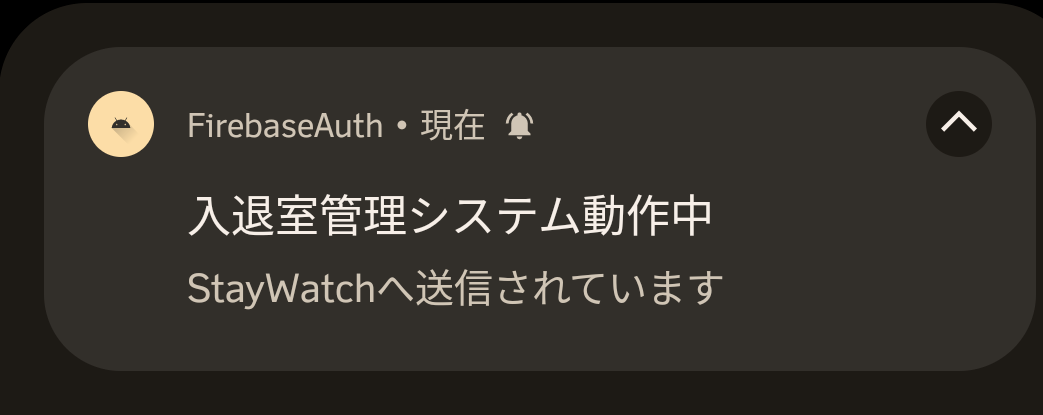
\includegraphics[width=12cm]{image/AppNofication.png}
  \caption{通知領域におけるビーコンの動作状況の表示}
  \label{fig:AppNofication}
\end{figure}


スマホビーコンは基本的にバックグラウンドに常在させる利用法を想定し実装した.
既存研究ではメンバに実デバイスによるビーコンを携帯させ,能動的な記録動作の必要がない.バックグラウンドに常在させる方式は実デバイスによるビーコンと同等の利便性がある.そのためバックグラウンドへの常在がアプリケーション化の前提である.
その点を踏まえて動作プラットフォームを選定した.
選定理由は技術調査をした際に,現状のiOSではフォアグラウンド動作はするもののバックグラウンド動作に制限がかかっており実デバイスによるビーコンと同等の利便性を担保することが困難であると判明したため,対応プラットフォームをAndroidのみにした.

実装に伴い,アプリケーションのプログラムはKotlinを用い,Bluetooth関連の実装においてはAltBeaconというライブラリを利用した.
選定した理由としては,Android標準のライブラリについての情報が少ない,一部公式ドキュメントが削除されている中,AltBeaconに関する情報が多く提供されているからである.
ビーコン動作をする上で,Androidのプライバシ規則によって,バックグラウンド上でのユーザへの通知無しでの動作は禁止されている.
その点と,先述のスマートフォンが表示機能を持つ点を利用して 図\ref{fig:AppNofication}に示す通り   通知領域上でビーコン動作中は常時表示する仕様とした.
この仕様によってユーザが入退室のたびにアプリの起動を行う必要もなく,プライバシ規則を遵守した上で,実デバイスによるビーコンと同様の能動的な記録動作を要しない利便性を担保した.

ビーコンのアプリケーション化に伴い,管理者が実デバイスによるビーコンで行っていた登録作業をより簡略化した.
従来では管理者が新しいメンバが増えるたびに登録作業をおこない,Googleアカウント,名前,UUIDなどを登録し,
それに合わせて実デバイスによるビーコンへ割り当てられたUUIDを登録する作業を行っていた.
しかし先述の通り,Firabaseによるログインによって,スマホビーコン上で利用するUUIDをメンバに紐づいているメールアドレスでログインすることで,利用できるようにした.

\newpage

% 手順は滞在WatchのWebページと同様である
\begin{figure}[tbh]
  \centering
  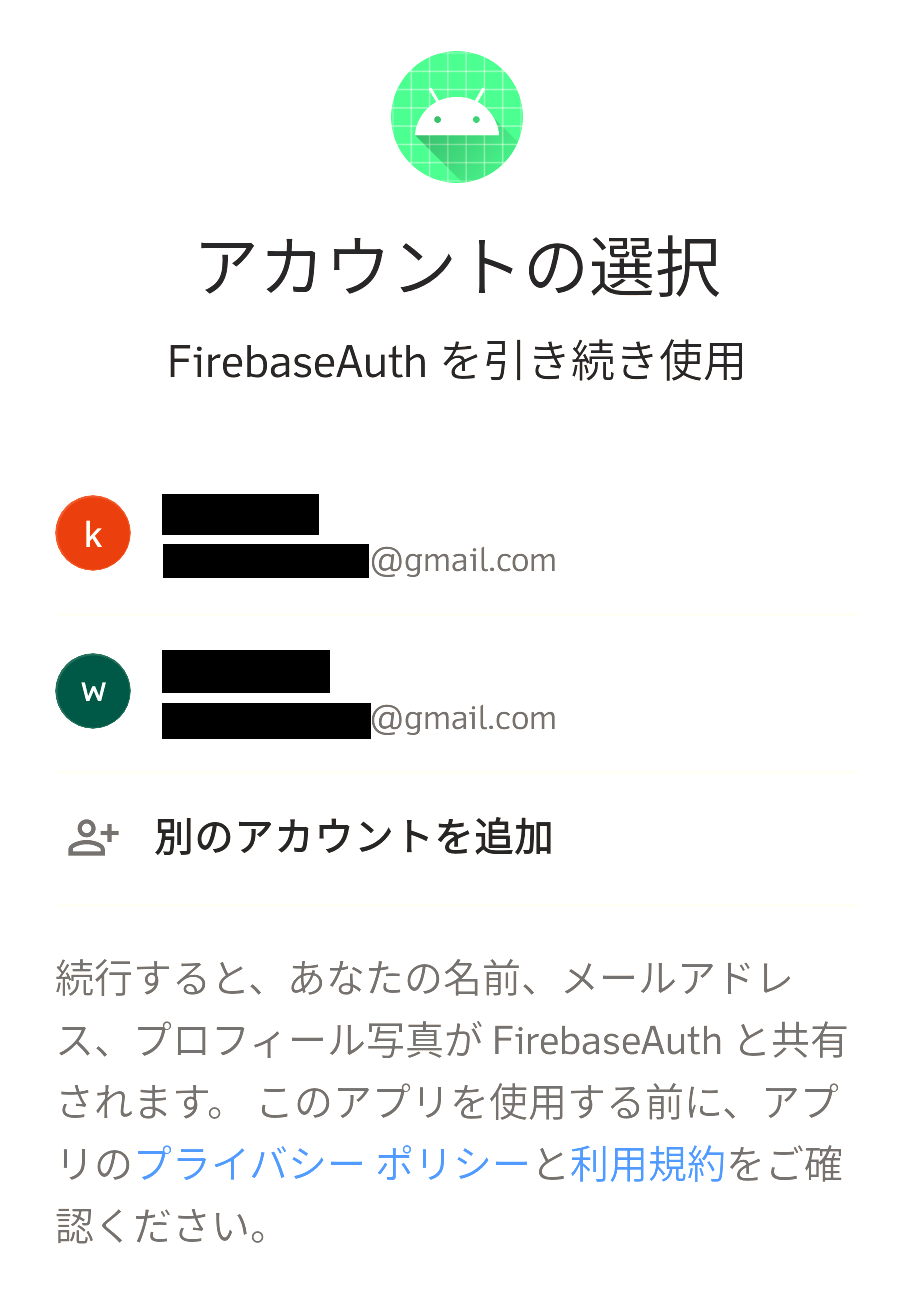
\includegraphics[width=9cm]{image/AppSignIn.png}
  \caption{アプリケーションのログイン画面}
  \label{fig:AppSignIn}
\end{figure}


図\ref{fig:AppSignIn}に示すサインインで管理者が登録したGoogleアカウントと一致する場合にログインを行う.その後APIからメンバの情報を受け取り,UUIDをアプリ内部に設定する.
以降はログイン時に受け取ったUUIDを用いたビーコン動作を行う.


% 画面の変更の写真を入れる
% \begin{figure}[tbh]
%   \centering
%   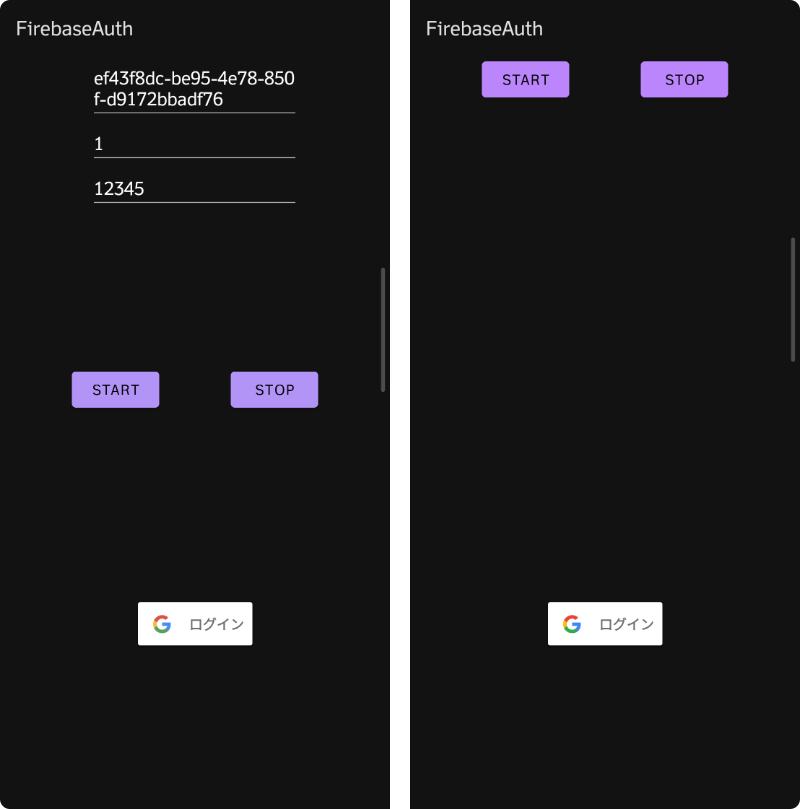
\includegraphics[width=9cm]{image/AppBeforeAfter.png}
%   \caption{メンバ向けアプリケーションにおける操作の簡略化}
%   \label{AppBeforeAfter}
% \end{figure}
% また図  X   研究初期はユーザから利用しているUUID,major,minorを編集できる仕様にしていたが,複雑な操作がユーザの利便性の向上につながらないと考え取り消した.
% あと,実デバイスによるビーコンでは管理者がユーザ登録を行ったあと紐づけたビーコンに一台ずつ対応したUUIDを割り当てていたが,スマホビーコンならばウェブ上に登録されたユーザに紐づいたUUIDを持ってくる
% 4.2章が完成したときに整合性を取ろう!!!